% ------------------
% -- Assignment 1 --
% -- Math 4171 -----

\documentclass[8pt,oneside]{book}

%\usepackage{subfigure}
\usepackage{subcaption}
\usepackage{graphicx}
\usepackage{amsmath}
\usepackage{amsfonts}
\usepackage{hyperref}
\usepackage{adjustbox}
\usepackage{listings}
\usepackage{xcolor}
\usepackage{titlesec}
\usepackage{enumitem}
\usepackage{mathrsfs}
\usepackage{anyfontsize}
\usepackage[driver=pdftex]{geometry}
\usepackage{import}
\usepackage{cleveref}
%\usepackage{titleformat{\section
%        {\normalfont\normalzie\bfseries}{Helo.}{1em}{}


\definecolor{codegreen}{rgb}{0,0.6,0}
\definecolor{codegray}{rgb}{0.5,0.5,0.5}
\definecolor{codepurple}{rgb}{0.58,0,0.82}
\definecolor{backcolour}{rgb}{0.95,0.95,0.92}
 
\lstdefinestyle{mystyle}{
    backgroundcolor=\color{backcolour},   
    commentstyle=\color{codegreen},
    keywordstyle=\color{magenta},
    numberstyle=\tiny\color{codegray},
    stringstyle=\color{codepurple},
    basicstyle=\fontsize{8}{10}\selectfont\ttfamily,
    breakatwhitespace=false,         
    breaklines=true,                 
    captionpos=b,                    
    keepspaces=true,                 
    numbers=left,                    
    numbersep=5pt,                  
    showspaces=false,                
    showstringspaces=false,
    showtabs=false,                  
    tabsize=2
}

\newtheorem{theorem}{Theorem}
\newtheorem{definition}{Definition}
\newtheorem{proof}{Proof}
 
\lstset{style=mystyle}

%\usepackage[margin=0.5in]{geometry}
%\usepackage{inputenc}

\newcommand{\Real}{\mathbb{R}}
\newcommand{\Int}{\mathbb{Z}}
\newcommand{\Nat}{\mathbb{N}}
\newcommand{\Complex}{\mathbb{C}}
\newcommand{\vect}[1]{\boldsymbol{#1}}

\renewcommand{\Re}[1]{\mathfrak{Re}\left\lbrace{#1}\right\rbrace}
\renewcommand{\Im}[1]{\mathfrak{Im}\left\lbrace{#1}\right\rbrace}

\title{{\bf Research Notes}\\\vspace{10pt}     
    \author{Jacques Nel}
}

\begin{document}

\maketitle

\chapter{Data collection}

For the daily stock ranking, we use End of Day US Stock Prices dataset published by Quotemedia.

The dataset columns are:
\texttt{date},
\texttt{open},
\texttt{high},
\texttt{low},
\texttt{close},
\texttt{volume},
\texttt{dividend},
\texttt{split},
\texttt{adj\_open},
\texttt{adj\_high},
\texttt{adj\_low},
\texttt{adj\_close}, and
\texttt{adj\_volume}.

\section{Downloading metadata--getting list of symbols}

The set of all symbols in the Quandl EOD dataset can downloaded at the following endpoint:

\begin{lstlisting}{language=Python}
META_ENDPOINT = 'https://www.quandl.com/api/v3/databases/EOD/metadata?api_key={}'
response = requests.get(META_ENDPOINT.format(settings.QUANDL_API_KEY))
\end{lstlisting}

From this CSV file, we extract the following columns: \texttt{qdl\_code},
\texttt{qdl\_name}, \texttt{qdl\_ticker}, and \texttt{qdl\_exchange}. On a few
occasions, \texttt{qdl\_code} can defer from \texttt{qdl\_ticker}. RegEx is used to parse HTML for
\texttt{qdl\_ticker} and \texttt{qdl\_exchange}.

\section{Filtering list of symbols}

\begin{figure}
    \caption{Diagram of ticker filtering}
    \includegraphics[scale=0.6]{filter.pdf}
\end{figure}

\subsection{Exchanges as denoted in Quandl EOD}

\begin{enumerate}
    \item NASDAQ
    \item NYSE
    \item NYSE MKT; now known as NYSE American, formerly AMEX; small cap equity market
    \item NYSE Arca; formely ArcaEx; mostly ETFs, ETNs, and ETVs
\end{enumerate}

We keep symbols from NASDAQ, NYSE, and NYSE MKT. NYSE Arca are discarded at moment, as it contains mainly
EFTs and similiar securities.

\subsection{NASDAQ symbol convention}\label{nasdaq_conv}

On NASDAQ a ticker might have a 5 letter name. The 5th letter conveys special meaning.

\begin{enumerate}
    \item A - class A shares
    \item B - class B shares
    \item C - NextShares ETMF (type of ETF)
    \item D - new issue
    \item E - denotes delinquiency in SEC filings
    \item F - foreign issue
    \item G - first convertible bond
    \item H - second convertible bond
    \item I - third convertible bond
    \item J - voting; temporarily denotes shareholder vote situation
    \item K - non-voting
    \item L - miscellaneous situation; seems to be bonds and preferred stock
    \item M - foruth preferred issue
    \item N - third preferred issue
    \item O - second preferred issue
    \item P - first preferred issue
    \item Q - indicates bankruptcy
    \item R - rights
    \item S - shares of beneficial interest
    \item T - securities with warrants or rights
    \item U - units
    \item V - when issued or when distributed; sahres that are set to split or similiar corporate action
    \item W - warrants
    \item X - mutual fund quoation service
    \item Y - american depository receipt
    \item Z - miscellaneous situations
\end{enumerate}

The following NASDAQ postfixes are treated as non-common stocks: \texttt{C, D, E, G, H, I, J,
L, M, N, O, P, Q, R, S, T, U, W, V, W, X}, and \texttt{Z}.

\emph{Note:} Special treatment is given to \texttt{GOOGL}, it ends in the 5-letter postfix \texttt{L}, but
breaks from the standard naming convention.

\subsection{NYSE symbol convention}

Similar to \cref{nasdaq_conv}, the following postfixes are treated as non-common securities:
\texttt{F, Q, I, Z, L, N, O, C, CL, P, WS, WD, U, V, W, R}, and \texttt{V}.

NYSE and NYSE MKT features dot, underscore, and 5-letter naming convention. In the case of dot or underscore
convention, the ticker is split into tokens delimited by \textbf{.} or \textbf{\_}. We examine the root for
known test tickers, and the last token for postfixes.

\subsection{Test tickers}

Some tickers are for internal exchange testing purposes, and must be filtered out.

\vspace{10pt}

NYSE test tickers: \texttt{ATEST}, \texttt{CTEST}, \texttt{MEST},
\texttt{NTEST}, \texttt{ZTST}, and \texttt{CBX}. 

\vspace{10pt}

NASDAQ test tickers: \texttt{ZAZZT}, \texttt{ZBZZT},
\texttt{ZJZZT}, \texttt{ZVZZT}, \texttt{ZXYZ\_A}, and \texttt{ZVZZCNX}.

With dot or underscore convention, both the whole ticker and the root token is examined.

\section{Indices as additional features}

\subsection{S\&P500 market index}

The S\&P500 market index, denoted \texttt{\$SPX} is scraped from Yahoo Finance. We use the following endpoint:
\begin{lstlisting}[language=Python]
endpoint = 'https://query1.finance.yahoo.com/v7/finance/download/%5EGSPC'
endpoint += '?period1={}&period2={}&interval=1d&events=history'
\end{lstlisting}

The API provides the following columns: \texttt{open, high, low, close, volume}, and \texttt{adj\_close}.
We can calculate an adjustment ratio $\kappa_a = \mathtt{adj\_close} / \mathtt{close}$. This allows us to
also calculate \texttt{adj\_open, adj\_high, adj\_low}, and \texttt{adj\_volume}.


\subsection{VIX market volatillity index}

The VIX market volatillity index, denoted \texttt{\$VIX} is scraped from Yahoo Finance. We use the following endpoint:
\begin{lstlisting}[language=Python]
endpoint = 'https://query1.finance.yahoo.com/v7/finance/download/%5EVIX'
endpoint += '?period1={}&period2={}&interval=1d&events=history'
\end{lstlisting}

We only use the \texttt{adj\_close} column.

\section{IB symbol lookup}

Interactive Brokers' TWS API allows one to query symbols in order to map ticker names to TWS contracts. This
is both a way to determine if a symbol is currently tradable, and enables one to capture high frequency 
tick level market data.

\section{Incremental database updates}

Quandl's Python API has bulk download functionality which can used to build a local database. The bulk
download can either be the whole EOD database, or a partial patch file to update dataset when it is a maximum of
1 day behind.

\begin{figure}
    \center
    \caption{Incremental update mechanism}
    \includegraphics[scale=0.3]{update}
\end{figure}

\subsection{Determining update type}

Past updates are tracked in a JSON file. A complete database rebuild is triggered under the following conditions:

\begin{enumerate}
    \item \texttt{qdl.sqlite3} database file not found.
    \item JSON update history file not found.
    \item JSON update history file currupted or invalid keys.
    \item No past updates.
    \item Version bump detected.
    \item Database is more than 1 day out of date.
\end{enumerate}

We can determine by how many days the database is out of date by using \texttt{pandas\_market\_calendars} to
count the number of trading days between the latest date in the sqlite3 database, and the latest date in
the patch file, downloaded via the Quandl API.

\begin{lstlisting}[language=Python]
# Get NYSE and NASDAQ trading days in current date range.
nyse = mcal.get_calendar('NYSE').schedule(start_date=last_date,
                                          end_date=newest_date)
nasdaq = mcal.get_calendar('NASDAQ').schedule(start_date=last_date, 
                                              end_date=newest_date)

# Check assumption that NYSE and NASDAQ have same calendars.
pd.testing.assert_frame_equal(nyse, nasdaq)

missing_days = len(nyse.index) - 1
\end{lstlisting}


\begin{figure}
    \center
    \caption{Determining update type}
    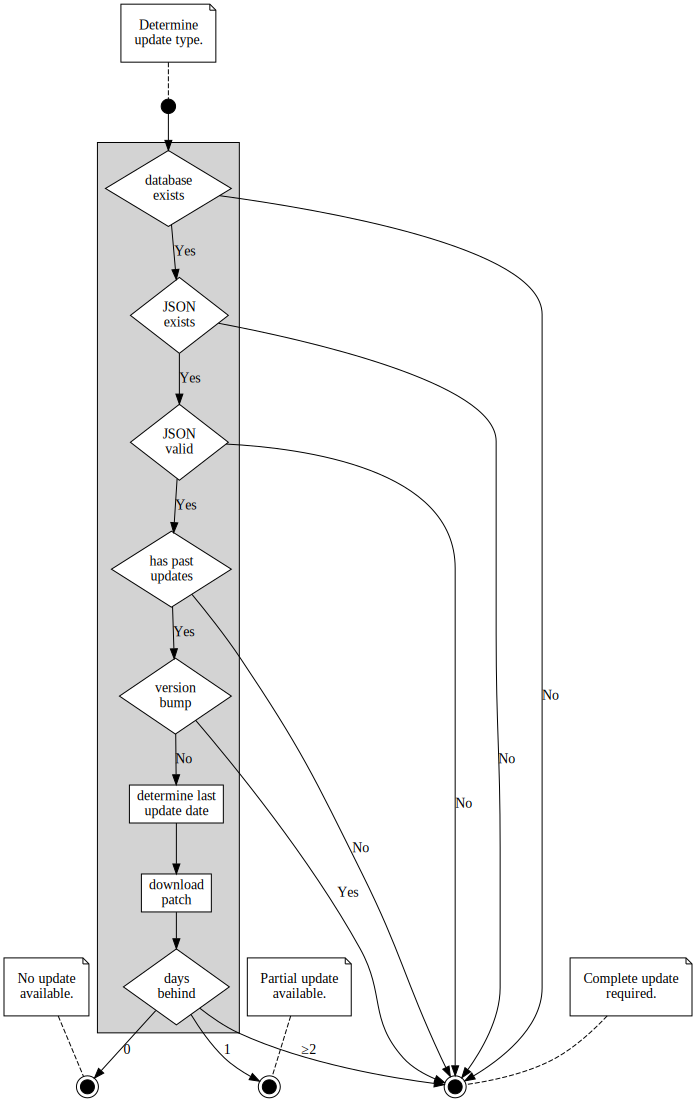
\includegraphics[scale=0.3]{update_type}
\end{figure}


\subsection{Complete database rebuild}

When we are forced to do a complete database rebuild, the entire EOD dataset must be downloaded via
the Quandl API. The following API call is used:

\begin{lstlisting}[language=Python]
quandl.bulkdownload('EOD',
                    api_key=settings.QUANDL_API_KEY,
                    download_type='complete')
\end{lstlisting}

The result is zip file in the current working directory (approximately 1Gb). The file is unzipped and its
records are
placed into the \texttt{qdl.sqlite3} database.

\begin{figure}
    \center
    \caption{Complete database rebuild}
    \includegraphics[scale=0.3]{complete}
\end{figure}

\subsection{Partial database patch}

When the database has been kept up to date, and all other conditions for partial update are met,
we can significantly speed up the database update, by only downloading a small patch file. The following
Quandl API call is used:

\begin{lstlisting}[language=Python]
quandl.bulkdownload('EOD',
                    api_key=settings.QUANDL_API_KEY,
                    download_type='partial')
\end{lstlisting}

The patch may include both new rows for new trading days, but also corrections and row updates (for things such
as adjustments, due to corporate action). New rows are simply appended. Retroactive updates are applied
by deleting matching old rows, and inserting new values.

\chapter{Realtime strategy}

\section{Feature engineering}

\subsection{Technical indicators}

\subsubsection{EMA}

A simple exponential moving average can be used to smooth the timeseries. Given some length $l$ and
smoothing parameter $\alpha$, we can calculate EMA as follows:

\begin{equation}
    \mathrm{EMA}_t = \left(x_t * \frac{\alpha}{1+l}\right) + \mathrm{EMA}_{t-1} * \left( 1 - \frac{\alpha}{1+l}\right)
\end{equation}

Since we require $\mathrm{EMA}_{t-1}$ at time step $t$, for $t=0$ we can simply use $\mathrm{EMA}_0 = x_0$, i.e.,
we initialize the moving average with the starting value of $\vect{x}$.

\subsubsection{MACD}

\emph{Moving Average Convergence Divergence} is a trend-following momentum indicator. It is calculated as
the difference between two moving avareges. Typically values are $l_1=12, l_2=26$, and $\alpha=0.5$, for
daily prices. It is simply calculated with

\begin{equation}
    \mathrm{MACD}_t = \mathrm{EMA}_t^{(1)} - \mathrm{EMA}_t^{(2)}
\end{equation}

It is common to smoothe the MACD signal by applying an EMA on its output. Buy/sell signals can be generated
by zero-crossings.

\subsubsection{Bollinger Bands}

\subsection{Probability distribution fitting}

\subsection{Heavy-tailed process}

The log returns of financial time series typically follow a heavy-tailed distribution. The probability
of extreme price swings fall off slowly.

The Lambert W transform can be used to model heavier-tailed process as in done in Quant GAN.


\section{Naive strategy}

\chapter{Reinforcement learning}

\section{Markov Decision Process}

\begin{figure}
    \center
    \caption{MDP example from David Silver's RL lectures}
    \includegraphics[scale=0.4]{mdp}
\end{figure}

A Markov decision process is defined as $(S,A,P_a,R_a)$ with

\begin{itemize}
    \item $S$ is the state space.
    \item $A$ is the action space; $A_s$ is the set of actions available
        in state $s$.
    \item $P_a (s, s' ) = Pr(s_{t+1} = s' | s_t = s, a_t =a)$ is the
        probability that action $a$ in state $s$ will lead to transition
        $s\rightarrow s'$ for timestep $t\rightarrow t+1$.
    \item $R_a(s,s')$ is the immediate reward received from the transition
        $s\rightarrow s'$ as result of action $a$.
\end{itemize}

\newpage

\section{REINFORCE}

The policy gradient equation is

\chapter{Actor Critic}

\begin{equation}
    \nabla_\theta J(\theta) = \mathbb{E}_\tau \left[
        \sum_{t=0}^{T-1}\nabla_\theta\log\pi_\theta\left(a_t|s_t\right)G_t\right]
\end{equation}


\begin{equation}
    \nabla_\theta J(\theta) = \mathbb{E}_\tau \left[
    \sum_{t=0}^{T-1}\nabla_\theta\log\pi_\theta\left(a_t|s_t\right)(G_t - b(s_t)\right]
\end{equation}

\begin{equation}
    \nabla_\theta(\theta)
    =
    \mathbb{E}_{s_0,a_0,\ldots,s_t,a_t}
    \left[\sum_{t=0}^{T-1} \nabla_\theta \log\pi_\theta(a_t|s_t)\right]
        \mathbb{E}_{r_{t+1},s_{t+1},\ldots,r_T,s_T}
        \left[G_t\right]
\end{equation}

Second term is the Q value.

\begin{equation}
    Q(s_t,a_t) = \mathbb{E}_{r_{t+1},s_{t+1},\ldots,r_T,s_T}
    \left[G_t\right]
\end{equation}

The update equation is then:

%\begin{equation}
%    \nabla_\theta J(\theta) =
%    \mathbb{E}_{s_0,a_0,\ldots,s_t,a_t}
%    \left[\sum_{t=0}^{T-1}
%    \nabla_\theta \log \pi_\theta(a_t|s_t)\right]
%    Q_w(s_t,a_t)
%    = \mathbb{E}_\tau\left[
%        \sum_{t=0}^{T-1}\nablda_\theta\log\pi_\theta
%    (a_t|s_t)Q_w(s_t,a_t)\right]
%\end{equation}

\textbf{Actor Critic} algorithms can be summarized as:

\begin{enumerate}
    \item The \emph{critic} estimates the value function; either
        action value $Q(s_t,a_t)$ or state value $V(s_t)$.
    \item The \emph{actor} update policy distribution $\pi_\theta(a_t|s_t)$
        in the direction suggested by \emph{critic}.
\end{enumerate}

\begin{figure}
    \center
    \caption{Actor Critic Algorithm}
    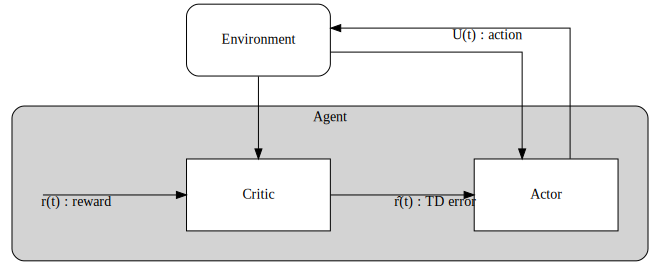
\includegraphics[scale=0.5]{actor_critic}
\end{figure}

The evaluation of the TD error is
\begin{equation}
    \delta_t = r_{t+1} + \gamma V(s_{t+1}) + V(s_t)
\end{equation}


\begin{equation}
    \pi_t(s,a) = Pr\left\lbrace a_t =0 | s_t =s \right\rbrace = \frac{e^{p(s,a)}}{\sum_b e^{p(s,b)}}
\end{equation}

\chapter{Discrete Soft Actor Critic}

\chapter{Planned future work}

\end{document}
